\section{Оформление иллюстраций}

В данном разделе приводится пример оформления иллюстраций по п.~2.3 ГОСТ~19.106 \cite{gost19106}.

Иллюстрации, если их в документе более одной, нумеруют арабскими цифрами в
пределах всего документа. В приложениях иллюстрации нумеруются в пределах каждого приложения аналогично как в основной части документа.

%\begin{figure}
%%	\vspace{5mm}
%%	\begin{center}
%		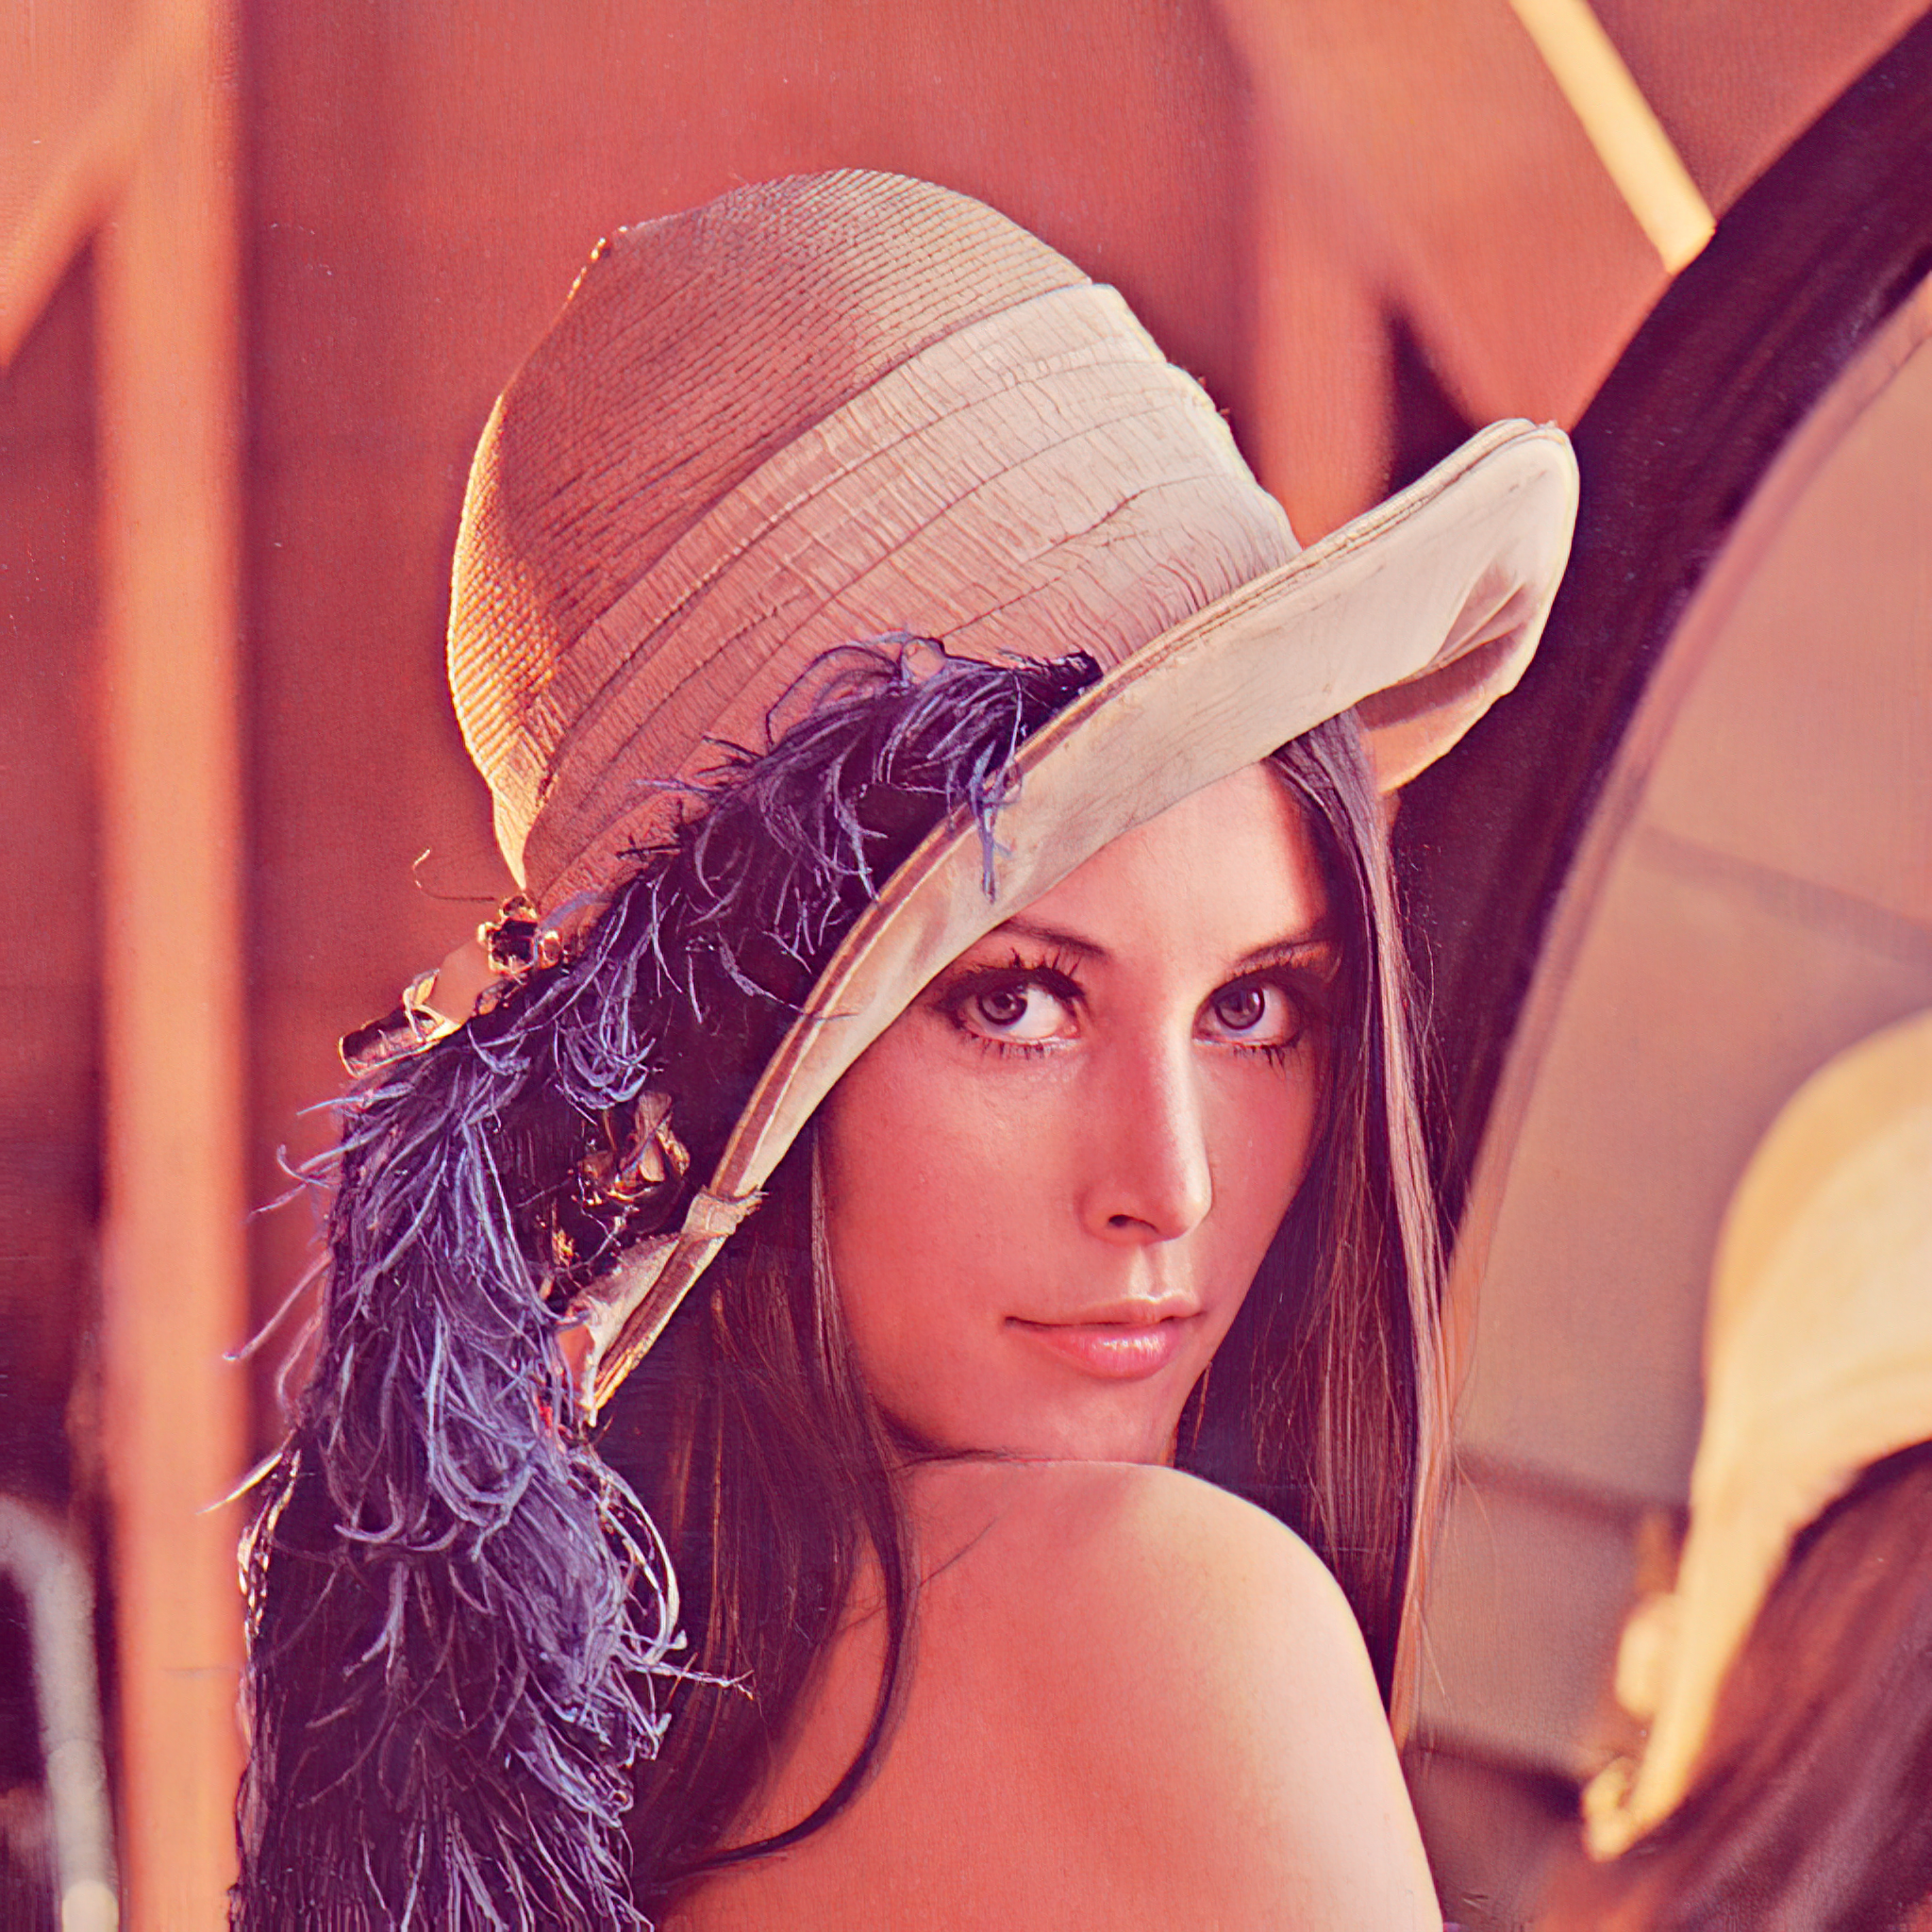
\includegraphics[width=0.5\textwidth]{Lenna}
%		\caption{Лена}
%%	\end{center}
%%	\vspace{5mm}
%%	\par
%\end{figure}

%\vspace{5mm}
%	\begin{center}
%		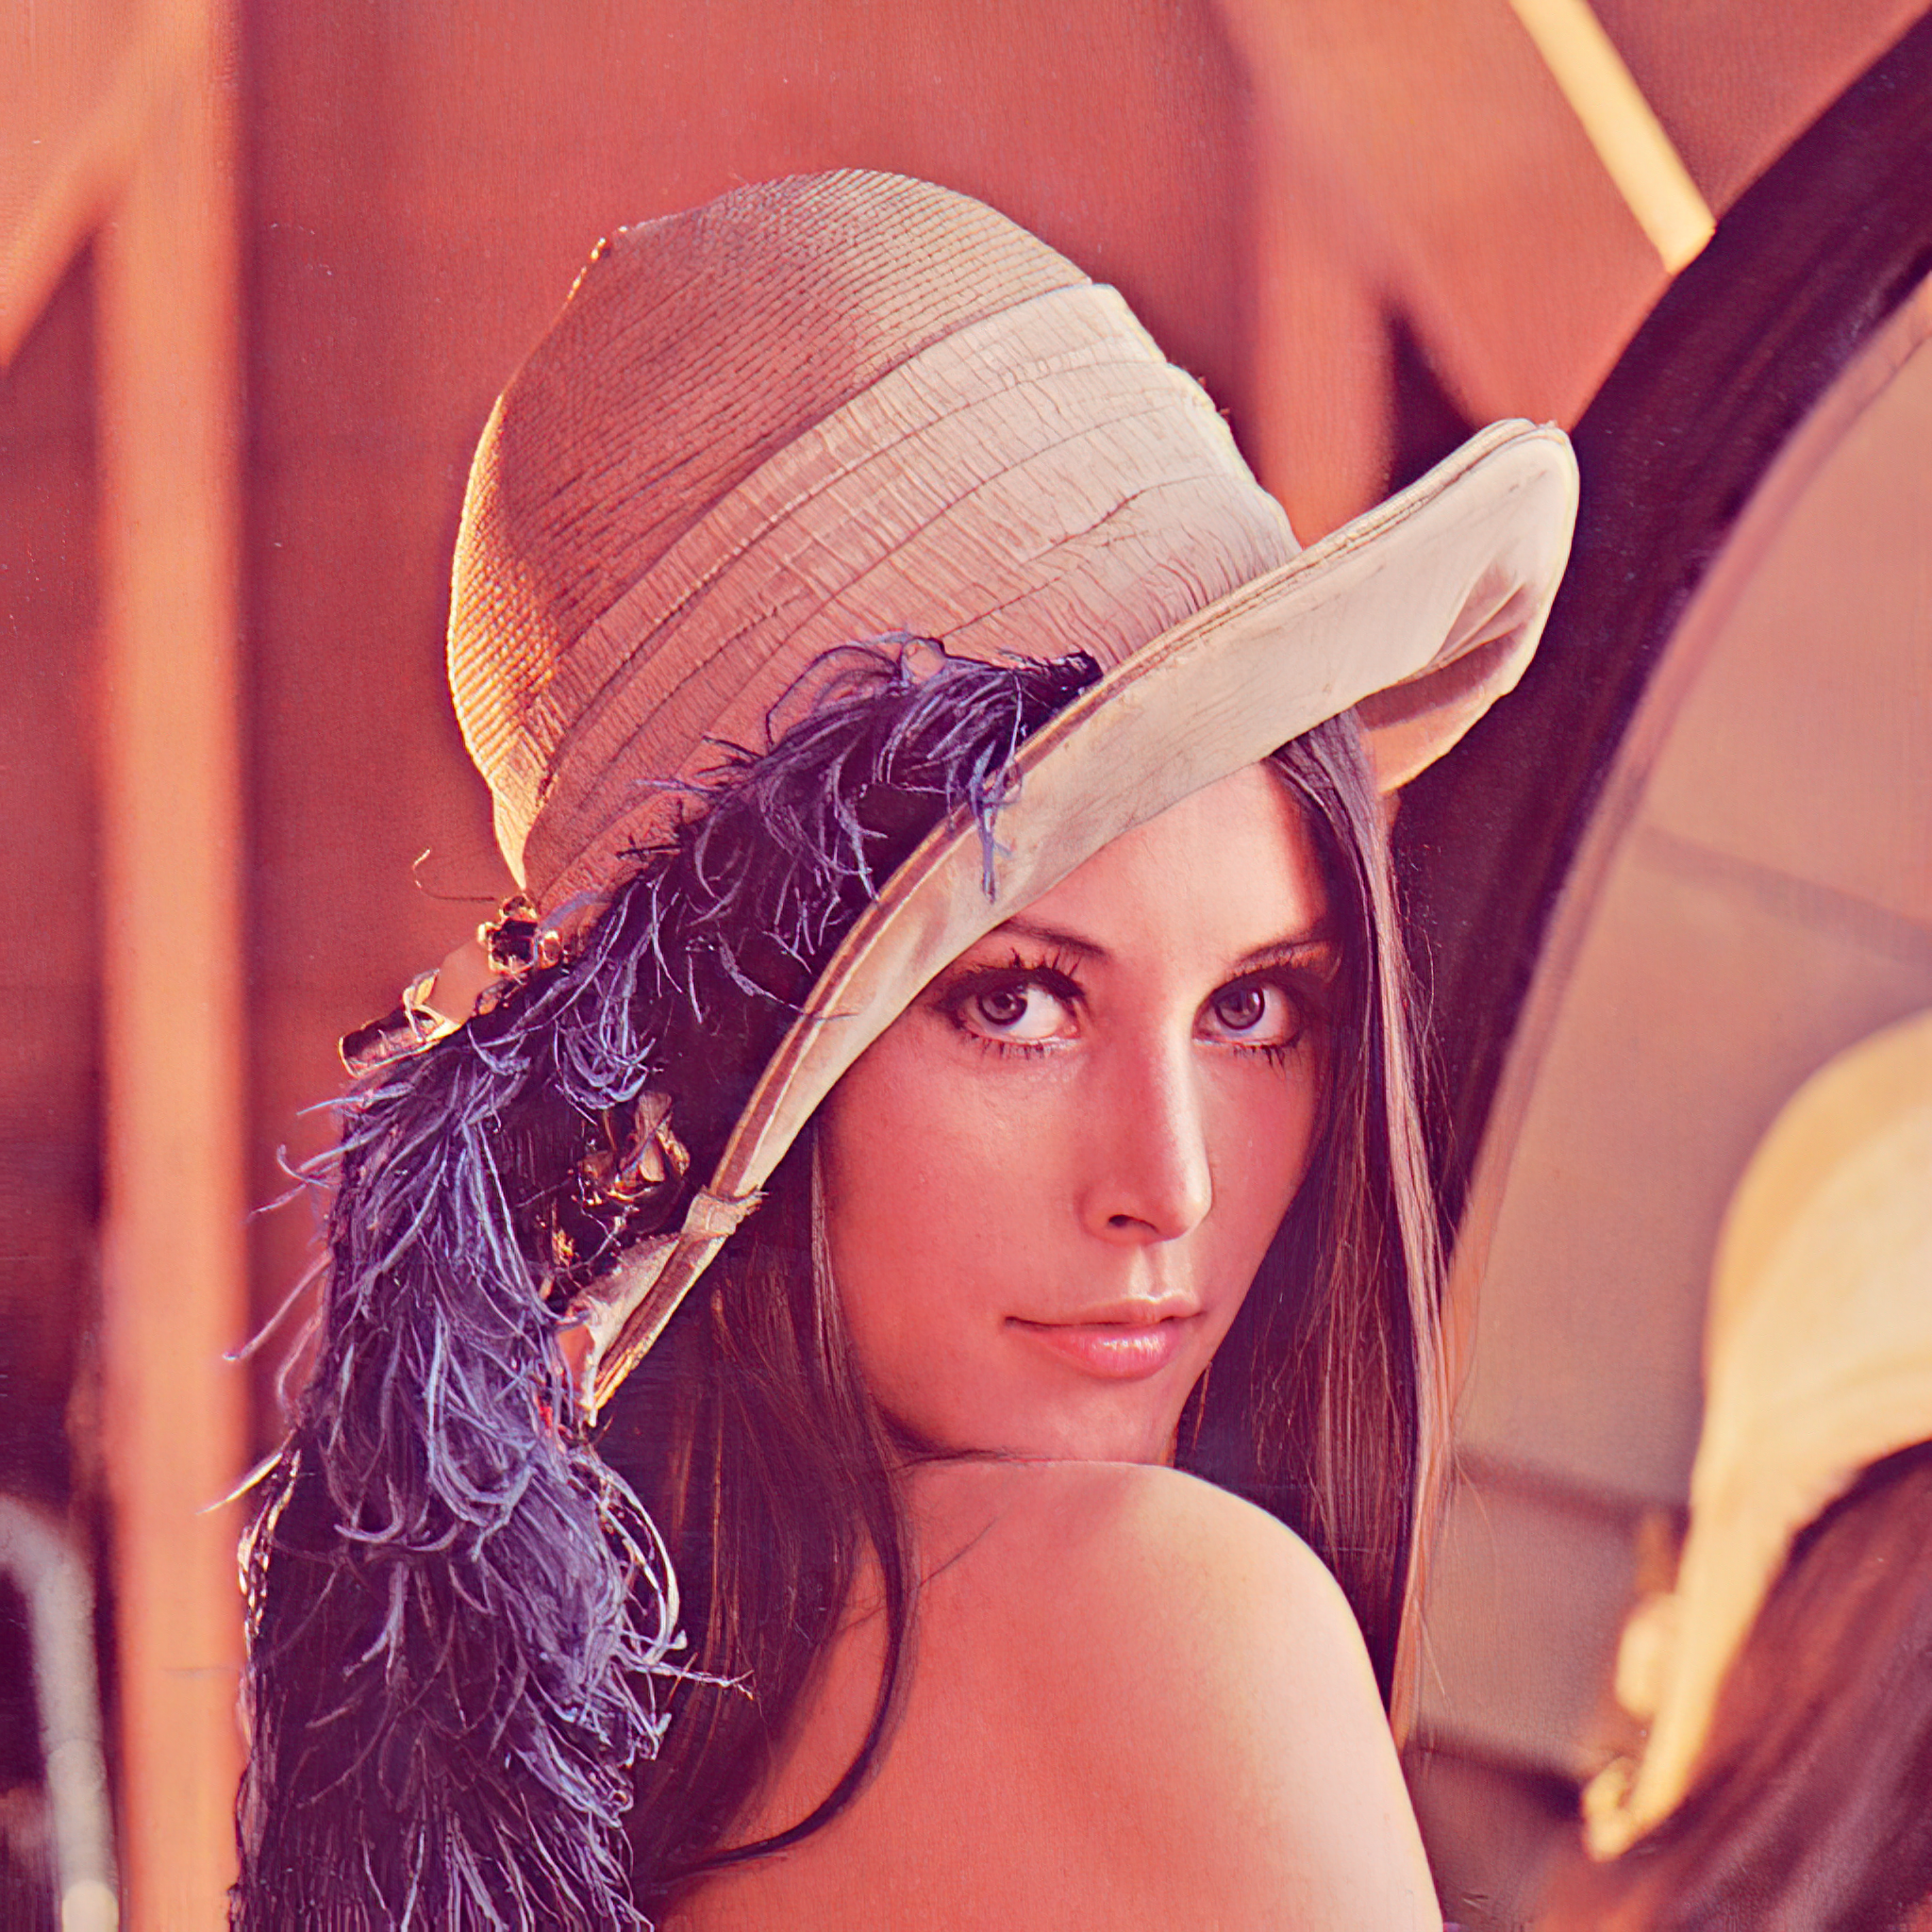
\includegraphics[width=0.5\textwidth]{Lenna}
%%		\caption{Лена}
%	\end{center}
%	\vspace{5mm}
%	\par



%\begin{figure}
%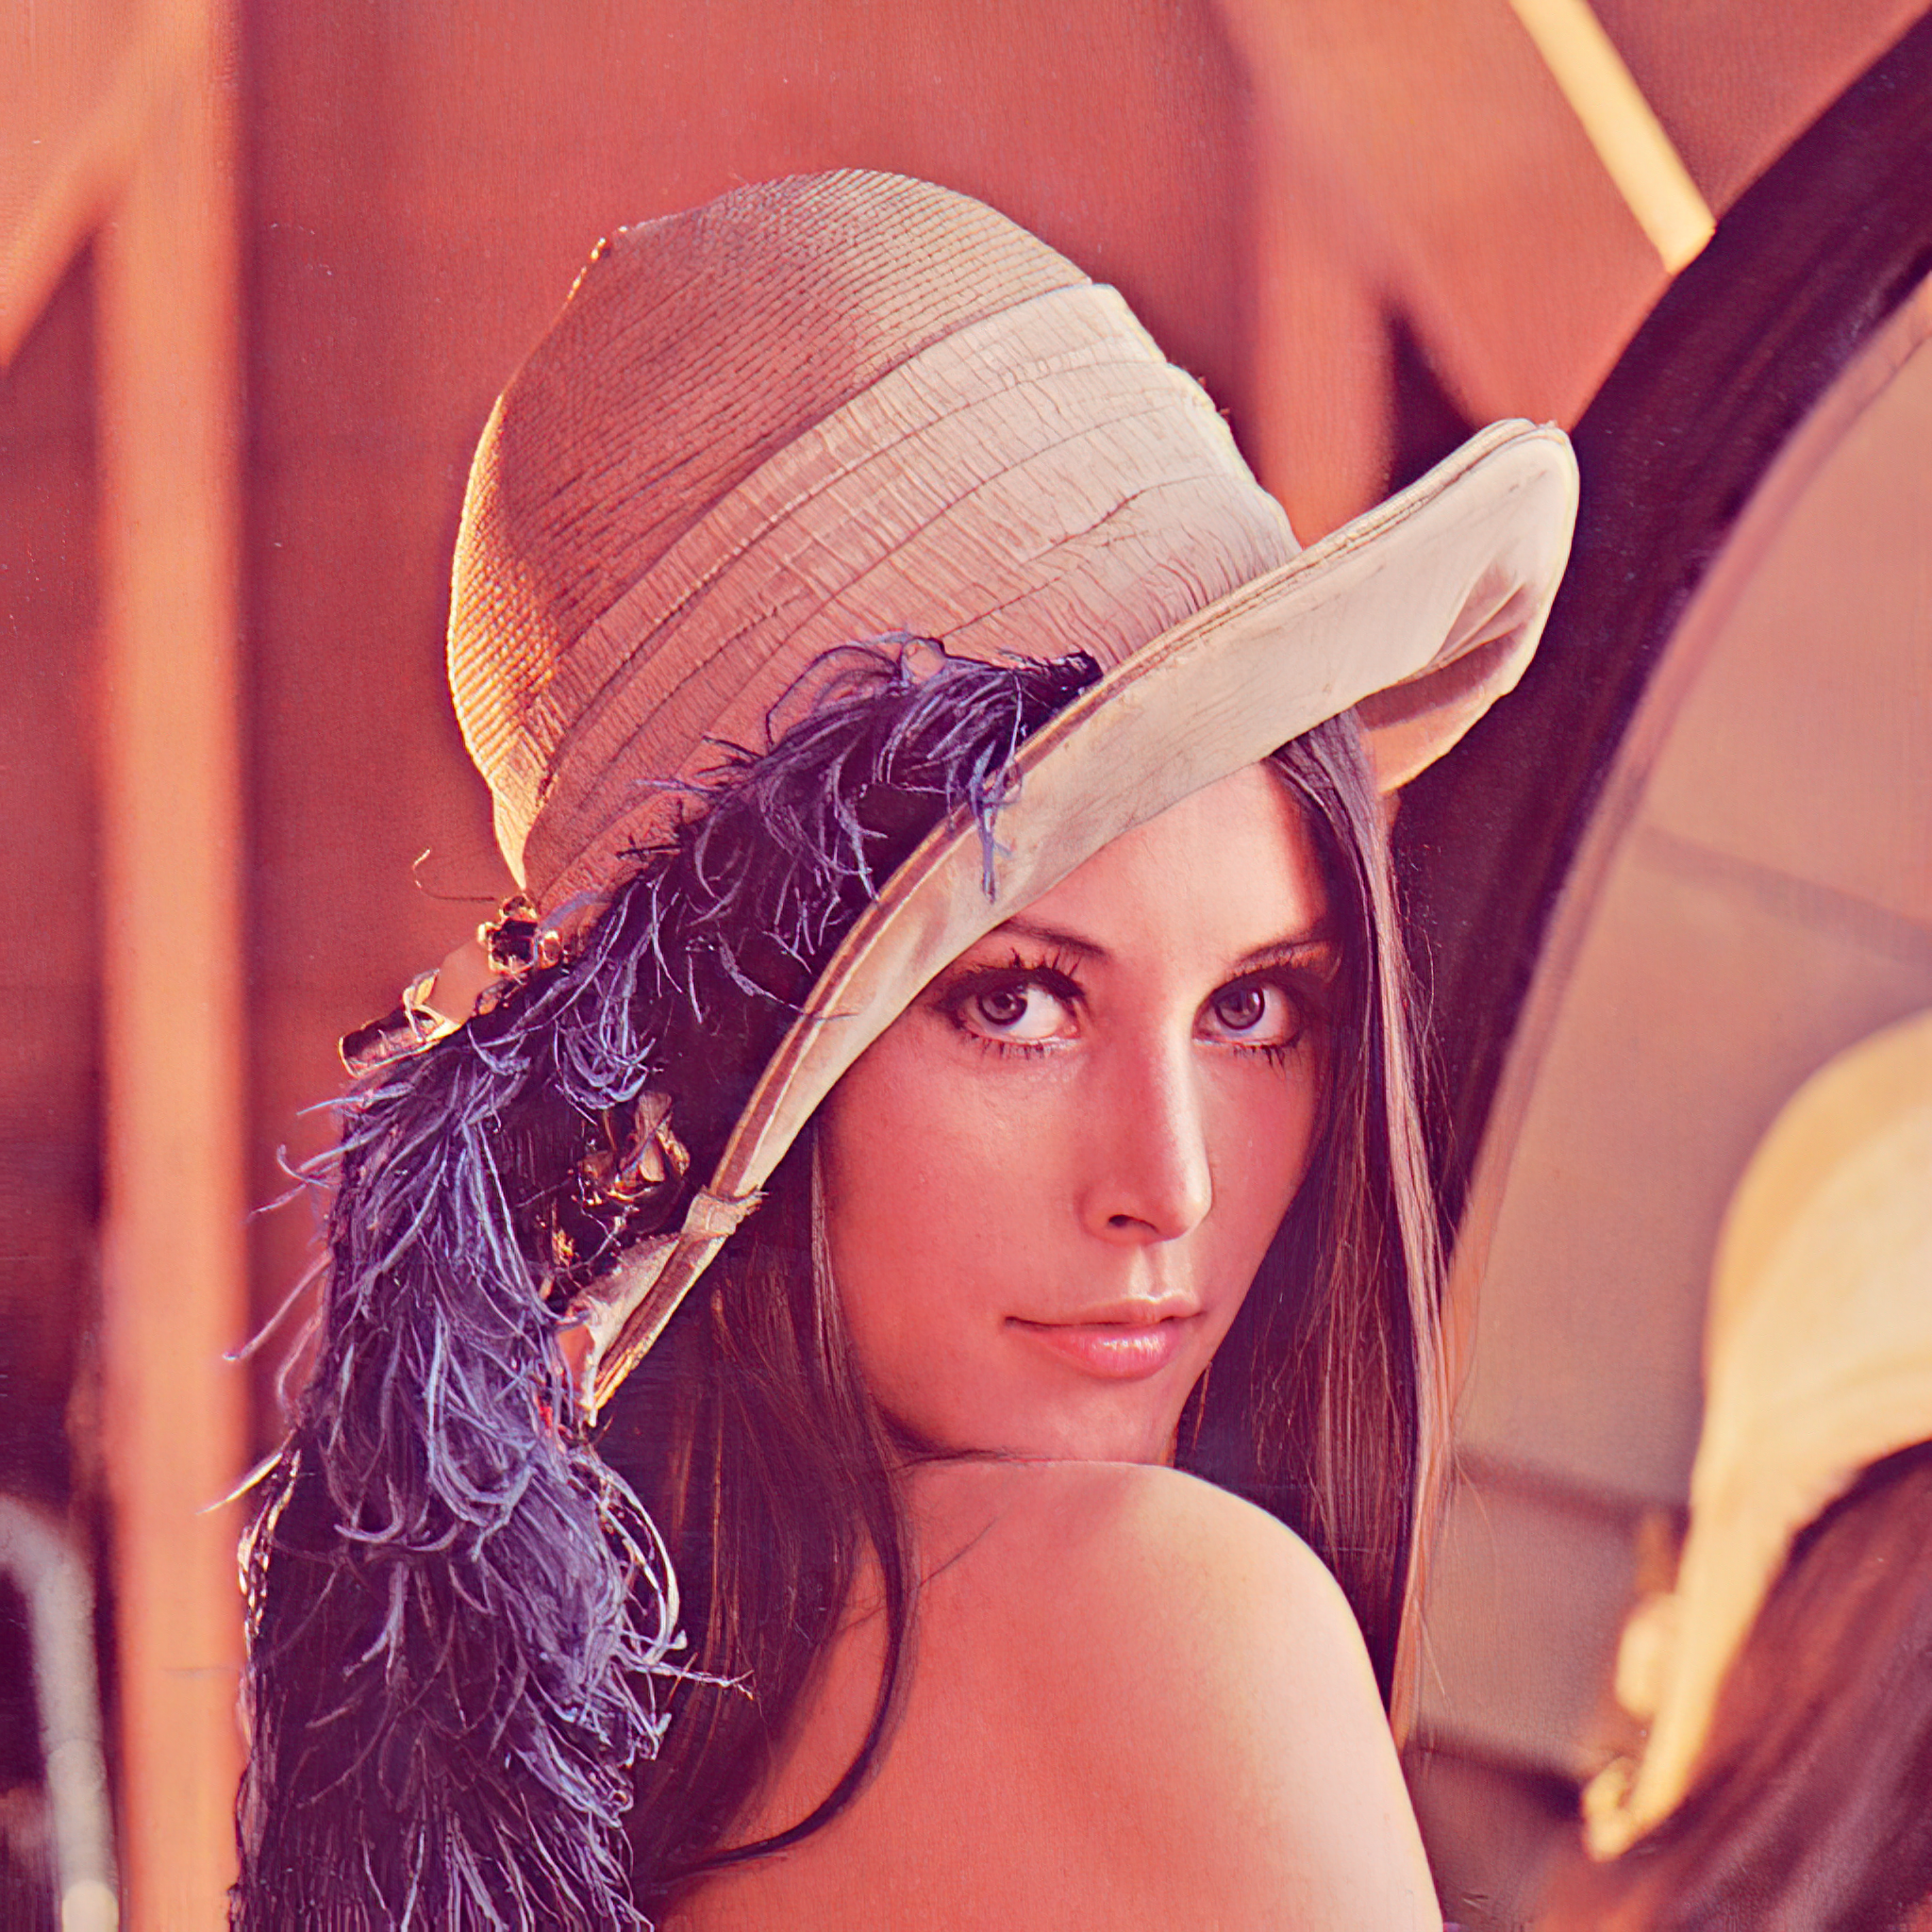
\includegraphics[width=8cm]{Lenna}
%\end{figure}
%\begin{figure}
%\image[0.5]{Lenna}
%\captionof{}{123}
%\caption{Caption}
%\label{fig:Лена}	
%\end{figure}
%
%\begin{figure}[h]
%	\centering
%	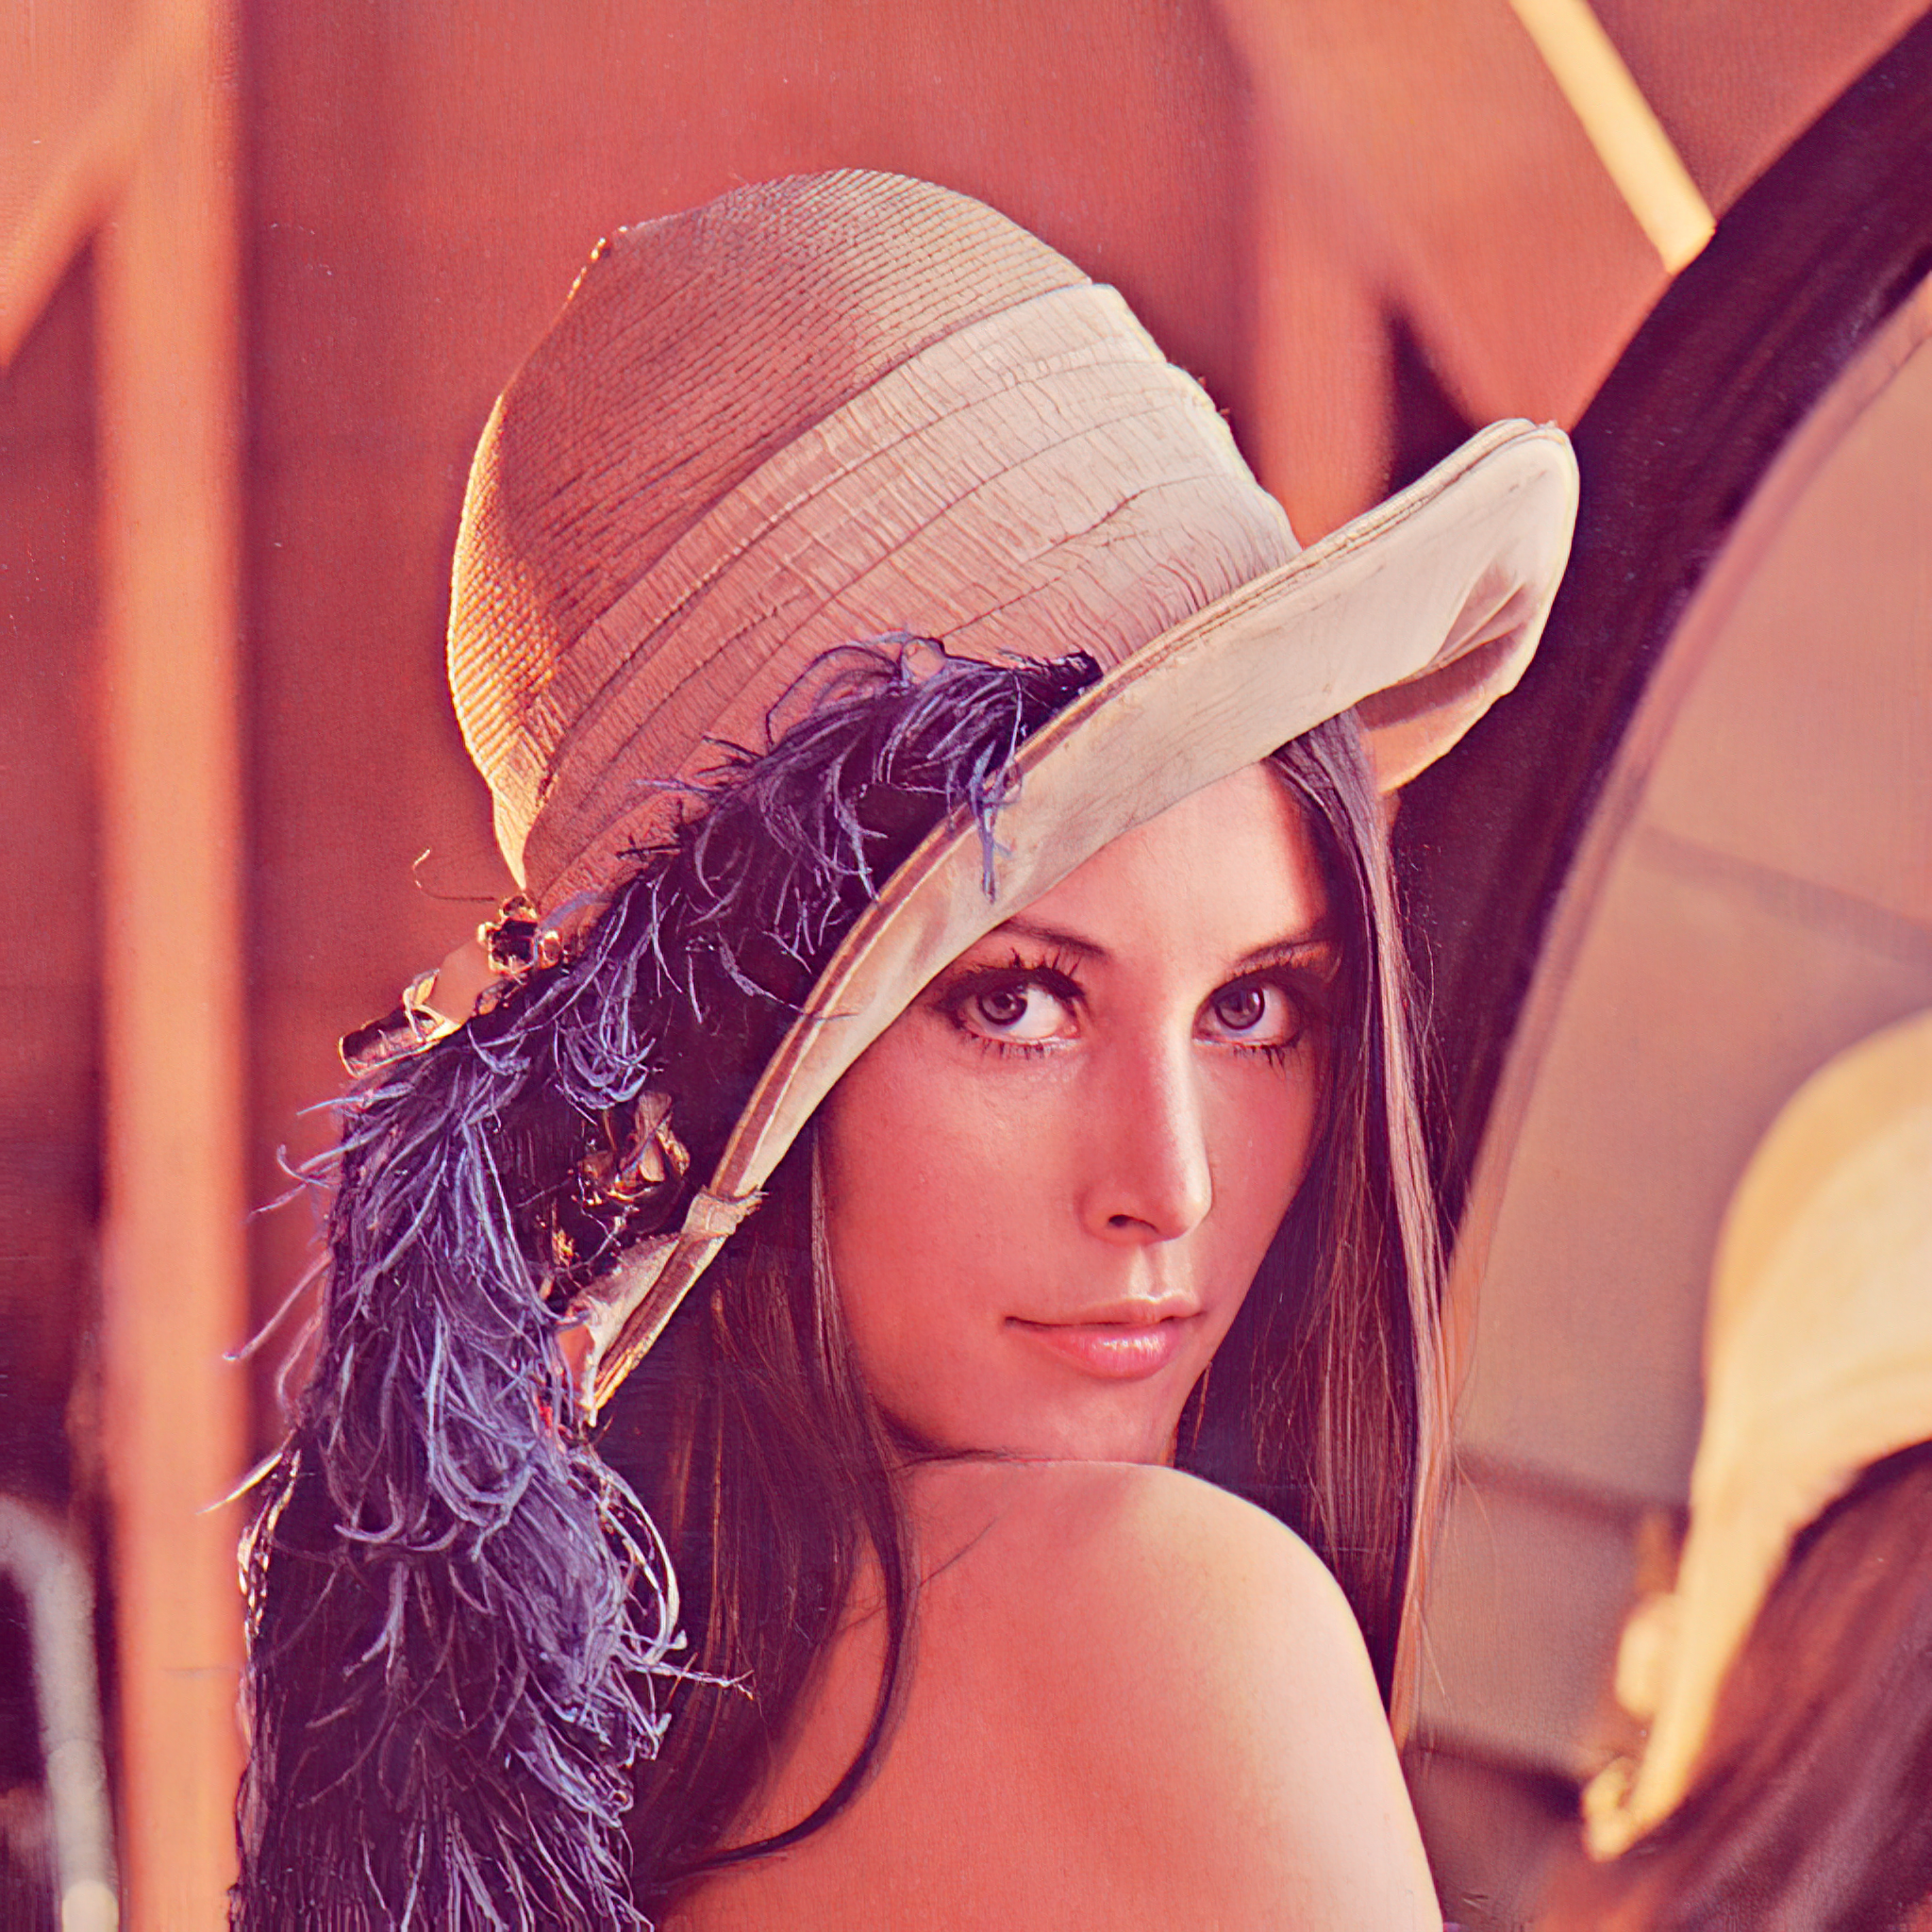
\includegraphics[width=\textwidth]{Lenna.png}
%%	\caption{Лена}
%%	\label{fig:Лена}
%\end{figure}
%
%

